\begin{figure}
 \centering
 \vspace{-1ex}
 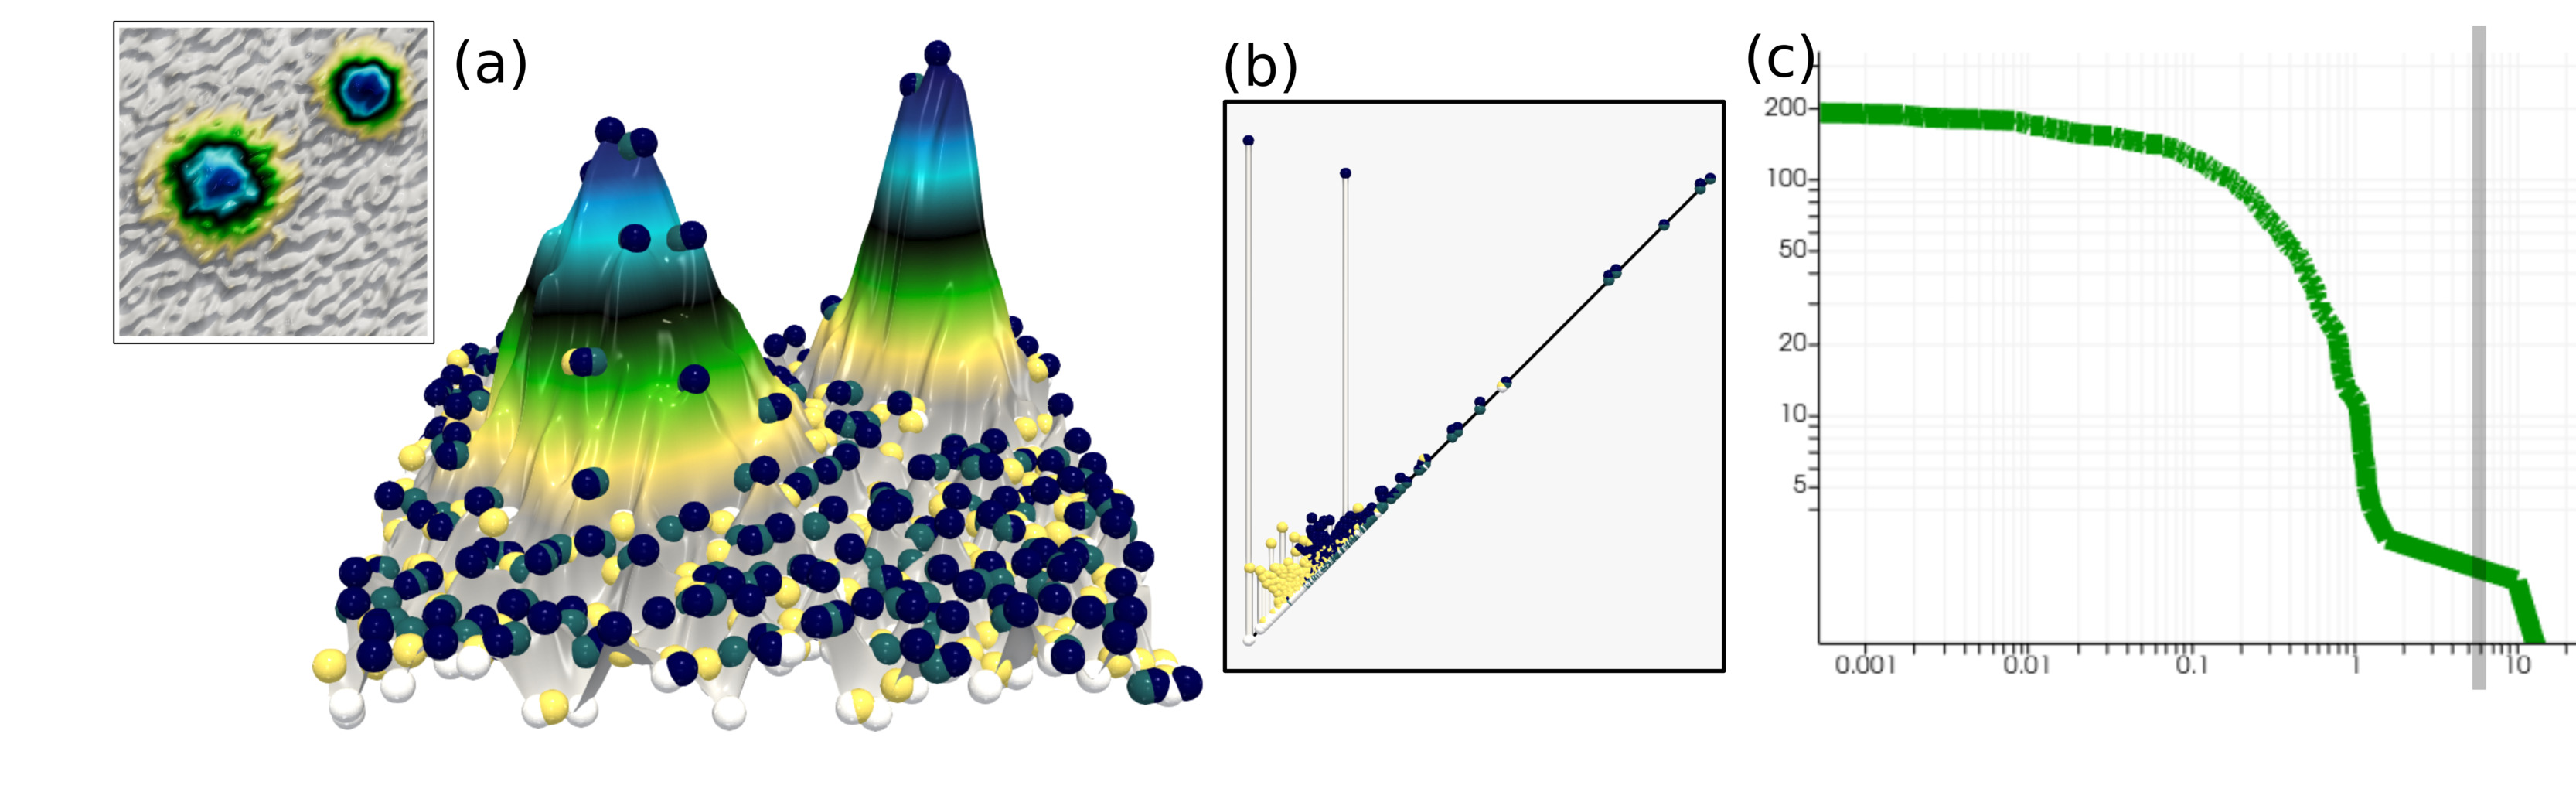
\includegraphics[width=\figureShrink\linewidth]{chapter4_topology_data_analysis/pictures/topo_gaussian.jpg}
 \caption{Critical points (spheres, white: minima, blue: maxima, other:
saddles), persistence diagram (b), persistence curve (c) of
a noisy (a) 2D
scalar field. The persistence diagram captures the main two hills of the
terrain as prominent persistence pairs (large vertical segments), while small
oscillations due to noise induce features near the diagonal.}
 \label{fig_toyTopology}
\end{figure}






\subsection{Topological data analysis}
\label{sec_topology}



This section presents the topological background of our work. It contains
definitions adapted from the Topology ToolKit \cite{ttk17}.
We refer the
reader to textbooks \cite{edelsbrunner09} for an introduction to
% computational
topology.

\noindent
\textbf{Input data.}
The input data is given as an ensemble of $N$ piecewise linear (PL) scalar
fields
$f_i : \domain \rightarrow \range$, with $i \in \{1, \dots,  N\}$, defined on a
PL 2-manifold $\domain$.
Specifically, $f_i$ represents the pointwise flow enstrophy
(\autoref{sec_simulation}) and $\domain$ is the Freudenthal triangulation
\cite{freudenthal42, kuhn60} of a $2$-dimensional regular grid, which is
periodic in both dimensions ($\domain$ is homeomorphic to a $2$-dimensional
torus). The triangulation is performed implicitly, by emulating the
simplicial structure upon traversal queries. Thus it induces no
memory overhead \cite{ttk17}.
The scalar values are given at the vertices of $\domain$ and are linearly
interpolated
on the simplices of higher dimensions.
$f$ is assumed to be injective on the vertices  of $\domain$.
This is
% easily
enforced in practice with a symbolic
perturbation inspired by Simulation of Simplicity \cite{edelsbrunner90}.


\noindent
\textbf{Critical points.}
Topological features in $f_i$ can be tracked with the notion of
\emph{sub-level set}, noted
$\sublevelset{{f_i}}(\isovalue)=\{p \in \domain~|
~f_i(p) < \isovalue\}$. It is defined as the pre-image of  $(-\infty,
\isovalue)$
by
$f_i$.
In particular, the topology of these sub-level sets (in 2D, their connected
components and cycles) can only change at special locations.
As $\isovalue$ continuously increases, the topology of
$\sublevelset{{f_i}}(\isovalue)$ changes at specific vertices of $\domain$,
called the \emph{critical points} of $f_i$ \cite{banchoff70}, defined next.
The \emph{star} of a vertex $v \in \domain$, noted $\Star(v)$,  is
the set of its co-faces:
$\Star(v) = \{ \simplex \in \domain ~|~ v < \sigma \}$.
It can be interpreted as the smallest combinatorial neighborhood around $v$.
The \emph{link} of $v$,
noted $\Link(v)$, is the set of the faces $\face$ of the simplices $\simplex$
of $\Star(v)$ with empty intersection with $v$:
$\Link(v) = \{ \face \in \domain ~ | ~ \face < \simplex, ~
\simplex\in \Star(v), ~ \face \cap v = \emptyset\}$.
The link of a vertex can
be interpreted as the boundary of its star.
The \emph{lower link} of $v$, noted $\lowerlink(v)$, is given by the
set of simplices of $\Link(v)$ which only contain vertices \emph{lower} than
$v$:
$\lowerlink(v) = \{ \simplex \in \Link(v) ~ | ~ \forall v' \in \sigma, ~ f_i(v')
< f_i(v)\}$. The upper link is defined symmetrically: $\upperlink(v) = \{
\simplex \in \Link(v) ~ | ~
\forall v' \in \sigma, ~ f_i(v') > f_i(v)\}$.
A vertex $v$ is \emph{regular}  if
and only if
both $\lowerlink(v)$ and $\upperlink(v)$ are simply connected. For
such vertices, the sub-level sets do not change their topology as they span
$\Star(v)$. Otherwise, $v$ is
a \emph{critical point}.
% of $f$ \cite{banchoff70}.
These can be classified with regard to their
\emph{index} $\Index(v)$.
It is equal to $0$ for local minima
($\lowerlink(v) = \emptyset$), to 2 for local maxima
($\upperlink(v) = \emptyset$) and otherwise to 1 for
saddles (\autoref{fig_toyTopology}a).
In practice, $f_i$ is enforced to contain only isolated, non-degenerate
critical points \cite{edelsbrunner90, edelsbrunner03}.
In the case of
the pointwise flow enstrophy, local maxima denote the center of vortices in the
turbulent flow. However, since the critical point characterization is based on a
classification which is only local (restricted to the link of each vertex), the
slightest oscillation in the data results in practice in the appearance of
spurious critical points, especially in the case of noisy data such as
turbulent flows. This motivates the introduction of an importance measure on
critical points, discussed next, in order to disambiguate vortices from noise.




\noindent
\textbf{Persistence diagrams.}
Several important
measures for critical points have been studied \cite{carr04},
including \emph{topological persistence} \cite{edelsbrunner02}, which is tightly
coupled to the notion of Persistence diagram \cite{edelsbrunner09}, which we
briefly describe here.
Persistence
assesses the importance of a critical point, based on the
lifetime of the topological feature it created (or destroyed) in
 $\sublevelset{{f_i}}(w)$, as one continuously increase the isovalue $w$.
In particular, as $w$ increases, new connected components of
$\sublevelset{{f_i}}(w)$ are created at the minima of $f_i$. The Elder rule
\cite{edelsbrunner09} indicates that if two connected
components, created at the minima $m_0$ and $m_1$ with $f_i(m_0) < f_i(m_1)$,
meet
at a given saddle $s$, the \emph{youngest} of the two components (the
one created at $m_1$) \emph{dies} in favor of the \emph{oldest} one (created at
$m_0$). In this case, a \emph{persistence pair} $(m_1, s)$ is created and
its
\emph{topological persistence} $p$ is given by $p(m_1, s) = f_i(s) - f_i(m_1)$.
All the local minima
can be
unambiguously
paired following this strategy, while the
global minimum is usually paired, by convention, with the global maximum.
The symmetric reasoning
can be applied to characterize, with saddle/maximum pairs, the life
time of the independent cycles of
$\sublevelset{{f_i}}(w)$.
Persistence pairs are usually
visualized with the \emph{Persistence diagram} $\diagram(f_i)$
\cite{edelsbrunner09}, which embeds each pair $(c, c')$, with $f_i(c) <
f_i(c')$,
as a point in the 2D plane, at location $\big(f_i(c), f_i(c')\big)$.
The  value $f_i(c)$ is 
% usually 
called the \emph{birth} of the
feature, while $f_i(c')$ is called its \emph{death}.
The
pair
persistence
can be
visualized as the height of the point to the diagonal.
Features with a high persistence stand out, away from the diagonal,
while noisy features are typically located in its vicinity 
(\autoref{fig_toyTopology}b).
The conciseness, stability \cite{edelsbrunner02} and expressiveness of this
diagram made it a popular tool
for data summarization tasks, as
it provides visual hints about the number, ranges and salience
of the features of interest.
To compare two datasets $f_i$ and $f_j$, persistence diagrams can be efficiently compared with the notion of $L_2$-Wasserstein distance \cite{CohenSteinerEH05,
Turner2014, Kerber2016} (we leave the practical study of distances between more
advanced topological descriptors  \cite{SridharamurthyM20,
pont_vis21} to future work). This distance is based on a bipartite assignment optimization problem (between the points of the two diagrams to compare), for which exact \cite{Munkres1957} and approximate \cite{Bertsekas81}
implementations are publicly available \cite{ttk17, ttk19}.
Specifically, we use in our approach the fast approximation scheme by Vidal et al. \cite{vidal_vis19}.
We refer the reader to \cite{Kerber2016, vidal_vis19, ttk19} for further
% practical
details.
Once the $L_2$-Wasserstein distance between two diagrams $\diagram(f_i)$ and $\diagram(f_j)$ is available (noted $\wasserstein{2}\big(\diagram(f_i), \diagram(f_j)\big)$), more advanced geometrical objects can be considered, such as \emph{Wasserstein barycenters} \cite{Turner2014, vidal_vis19}, which are
% representative
diagrams minimizing the sum of their distance to an ensemble of diagrams, and which consequently, can be considered as a reliable representative of the ensemble.
This notion of \emph{barycenter}
% it
is conducive to the design of clustering algorithms.
% , directly in
% the Wasserstein metric space.
% In particular,
The $k$-means algorithm
% \cite{elkan03, celebi13}
can be easily extended,
by using $\wasserstein{2}$ to measure distances between diagrams, and by
considering as cluster centroid, at each iteration of the $k$-means, the
 barycenter of the cluster.


\noindent
\textbf{Persistence curves.}
A popular, alternate, representation of persistence features is the notion of
\emph{Persistence Curve}, noted $\persistentCurve(f_i)$, which plots the
population of persistent pairs as a function of their persistence.
Specifically, it encodes the number of pairs (Y axis) whose persistence is
\emph{larger} than a threshold $\epsilon$ (X axis).
For $X=0$, $Y$ is equal to the total number of persistence pairs, while for the
largest values of $X$, $Y$ indicates the number of prominent, high-persistence
features (\autoref{fig_toyTopology}c).
In practice, large
plateaus in this curve will indicate \emph{stable} persistence ranges, for
which no (or few) topological features are present in the data. These 
correspond to \emph{separations} (vertical line, \autoref{fig_toyTopology}c) 
between populations of topological
features of distinct persistence scales, typically the noise (low $X$
values) and the persistent features (high $X$ values).

